% 使用 tkz-euclide 绘图的代码
\begin{tikzpicture}
	\tkzDefPoints{-0.7/0/M, 0/0/A, 0.7/0/N, 1/0/B, 1.5/0/C}
	\tkzDrawLine[add=0.8 and 0.5](A,C)
	\tkzLabelLine[pos=1.5,right](A,C){$l$}
	\tkzDrawPoints[fill=black](A,B,C,M,N)
	\tkzLabelPoints[above](A,B,C)
\end{tikzpicture}

% 下面是直接使用 tikz 绘图的代码,放在这里作对比
% \begin{tikzpicture}
% 	\coordinate (A) at (0,0);
% 	\coordinate (B) at (1.0,0);
% 	\coordinate (C) at (1.5,0);
% 	\coordinate (M) at (-0.7,0);
% 	\coordinate (N) at ( 0.7,0);

% 	\draw (-1.2,0) -- (2.25, 0) node[right] {$l$}; % AC长 1.5, 1.5+1.5*0.5=2.25;  1.5*0.8=1.2
% 	\foreach \x in {A,B,C,M,N} {
% 		\draw[fill=black] (\x) circle (1pt);
% 	}
% 	\foreach \x in {A,B,C} {
% 		\draw (\x) node [above] {$\x$};
% 	}
% \end{tikzpicture}

